%%%%%%%%%%%%%%%%%%%%%%%%%%%%%%%%%%%%%%%%%%%%%%%%%%%%%%%%%%%%%%%%%%%%%%%%%%%%%%%
\input{addons/lab-head}  % преамбула
\usepackage{wrapfig}
%%%%%%%%%%%%%%%%%%%%%%%%%%%%%%%%%%%%%%%%%%%%%%%%%%%%%%%%%%%%%%%%%%%%%%%%%%%%%%%

\newcommand{\labauthors}{Сарафанов Ф.\,Г}%., Сидоров Д.\,А.}
\newcommand{\labauthor}{Сарафанов~Ф.\,Г.}
\newcommand{\labnumber}{27}
\newcommand{\labtheme}{Определение отношения заряда электрона к его массе}

\newcommand{\ddt}{$\ \pm\ 0.2\ \text{с}$}
\newcommand{\ddtv}{$\ \pm\ 0.8\ \text{с}$}
\newcommand{\ddh}{$\ \pm\ 0.1\ \text{см}$}
\newcommand{\dm}{\Delta{}m}
\newcommand{\Dh}{\Delta{}x}
\newcommand{\Dl}{\Delta{}(\lambda)}
\newcommand{\dmsr}{<\Delta{}m>}
\newcommand{\el}{\varepsilon(\lambda)}
\newcommand{\F}{\vec{F}}
\newcommand{\A}{\vec{a}}
\newcommand{\E}{\vec{E}}
\newcommand{\B}{\vec{B}}
\newcommand{\V}{\vec{v}}

%%%%%%%%%%%%%%%%%%%%%%%%%%%%%%%%%%%%%%%%%%%%%%%%%%%%%%%%%%%%%%%%%%%%%%%%%%%%%%%
\input{addons/lab-kol} % колинтулы на страницах
%%%%%%%%%%%%%%%%%%%%%%%%%%%%%%%%%%%%%%%%%%%%%%%%%%%%%%%%%%%%%%%%%%%%%%%%%%%%%%%

\begin{document}

	\begin{titlepage}

	\begin{center}

	{\small\textsc{Нижегородский государственный университет имени Н.\,И. Лобачевского}}
	\vskip 1pt \hrule \vskip 3pt
	{\small\textsc{Радиофизический факультет}}

	\vfill

	{\Large Отчет по лабораторной работе №\labnumber\vskip 12pt\bfseries \labtheme}
		
	\end{center}

	\vfill
		
	\begin{flushright}
		{Выполнил студент 410 группы\\\labauthor\vskip 12pt Принял:\\ Менсов С.\,Н.}
	\end{flushright}
		
	\vfill
		
	\begin{center}
		Нижний Новгород, 2016
	\end{center}

	\end{titlepage}

\section{Отчёт по лабораторной работе №\labnumber \\ <<\labtheme>>}

% \subsection{Физические основы лабораторной работы}

В лабораторной работе исследуется равноускоренное движение на установке <<машина Атвуда>>.

Погрешности, используемые в работе: погрешность секундомера ---  $\Delta\,t=0.01\ c$, погрешность измерения длины ---  $\Delta\,h=0.5\ \text{см}$, погрешность известной массы грузов $M$ ---  $\Delta\,M=0.5\  \text{г}$, погрешность масс перегрузков $m_1, m_2$ --- $\Delta\,m=0.05\  \text{г}$.

Запишем 2 закон Ньютона для грузов $M+m_1$ (слева) и $M+m_1$ (справа):

\begin{EqSystem}
	(M+m_1)\vec{a_1}=(M+m_1)\vec{g}+\vec{T_1}\\
	(M+m_2)\vec{a_2}=(M+m_2)\vec{g}+\vec{T_2}
\end{EqSystem}

Спроецируем на ось X, направленную вертикально вниз:

\begin{EqSystem}
	\label{eq:ax}
	(M+m_1){{a_1}_x}=(M+m_1){g}-{T_1}\\
	(M+m_2){{a_2}_x}=(M+m_2){g}-{T_2}
\end{EqSystem}

% \begin{equation}
% X(\omega) = 
%  \begin{cases}

%  \end{cases}
% \end{equation}

Нить предполагается невесомой. Тогда можно записать 2 закон Ньютона для участка нити длиной $\Delta\,L\rightarrow0$. На участок цепи действуют силы натяжения нити и тормозящая сила %(см. рис. \ref{}):

\begin{gather}
	\label{eq:dl}
	F=ma\\
	m\vec{a_{\Delta\,L}}=\vec{F_\text{т}}+\vec{T_1}+\vec{T_2}
\end{gather}

Из условия невесомости масса участка равна нулю. Учитывая это, запишем проекцию (\ref{eq:dl}) на ось X:

\begin{gather}
\label{eq:TTF}
	T_2-T_1=F_\text{т}
\end{gather}

Однако, из третьего закона Ньютона можно обобщить это равенство на произвольную длину нити, так как на каждом участке силы будут транзитивно равны силе, приложенной от предыдущего участка нити.

Рассмотрим нерастяжимую нить. Сдвинем без ускорения нить на $\Delta\,x$ за время $\Delta\,t$. Из условия нерастяжимости грузы пройдут равное расстояние по модулю, но противоположное по направлению. Запишем скорость этих точек по определению: 

\begin{gather}
	\label{eq:dx}
	v_{1x}=\frac{\Delta\,x}{\Delta\,t},	v_{2x}=\frac{-\Delta\,x}{\Delta\,t}\Rightarrow\\
	v_{1x}=-v_{2x}
\end{gather}

Возьмем производную по времени от скорости (\ref{eq:dx}), по определению это будет проекция ускорения грузов на ось X:

\begin{gather}
	v_{1x}=-v_{2x}\\
	\frac{d}{dt}{v_{1x}}=-\frac{d}{dt}{v_{2x}}\\
	a_{1x}=-a_{2x}\label{eq:dv}
\end{gather}

Перепишем систему уравнений (\ref{eq:ax}) с учетом невесомости (\ref{eq:TTF}) и нерастяжимости (\ref{eq:dv}) нити:

\begin{equation}
\begin{cases}
	(M+m_1){-{a_2}_x}=(M+m_1){g}-{T_1}\\
	(M+m_2){{a_2}_x}=(M+m_2){g}-{T_1+F_\text{т}}\label{eru2}
 \end{cases}
\end{equation}

Выразим отсюда ускорение, вычитая уравнения в системе (\ref{eru2}):

\begin{gather}
	\label{eq:a2x}
	a_{2x}=\frac{(m_2-m_1)g-F_\text{т}}{2M+m_1+m_2}
\end{gather}

Как видно из уравнения (\ref{eq:a2x}), ускорение блоков зависит от тормозящей силы. Для того, чтобы применить это уравнение, необходимо найти физический смысл этой силы и её зависимость от известных величин.

% Можно предположить, что в силе трения есть свободный член $F_0$, неизменный во времени. Неизменно во времени сухое трение. 

% Итак, член $F_0$ -- это  сухое трение в установке.

Можно выдвинуть несколько гипотез о тормозящей силе : $F_\text{т}=F_0+?$

\subsection{Гипотеза первая. $F_\text{т}=F(v)$}
Тормозящая сила зависит от скорости, где-то возникает вязкое трение. Это можно проверить, сняв зависимость $h(t^2)$ для разных перегрузков. 

Рассчитаем прямоугольники погрешностей измерений.

\begin{gather*}
	\Delta\,h=0.5\ \text{cm}\\
	\Delta\,(t^2)=2t\Delta\,t
\end{gather*}

% Максимальная абсолютная погрешность времени составляет для максимального замеренного времени $\tau=4.49$ секунды $\Delta\,(\tau^2)=2\cdot4.49\cdot0.01=0.08$ секунды, откуда следует, что изобразить прямоугольники погрешностей на графике (\ref{fig1}) на данном масштабе нельзя. 

\begin{figure}[h]
\begin{center}
\includegraphics*[width=1\textwidth]{img/ex1.png}
\caption{\label{fig1}Эскиз графика зависимости $h(t^2)$}
\end{center}
\end{figure}

Как видно из графика, все три груза двигались с постоянным ускорением --- следовательно, гипотеза $F_\text{т}=F(v)$ неверна. 

% На графике видно небольшое отклонение от прямой больше размера прямоугольника погрешностей. Это опыты, в которые была внесена ошибка измерения. Предположительно --- из-за магнита, который отрывал груз в разное, отличное от начального, время.

\subsection{Гипотеза вторая. $F_\text{т}=F_0+F(a)=F_0+\lambda{}a$}

Перепишем уравнение (\ref{eq:a2x}) с учетом $F_\text{т}=F_0+F(a)=F_0+\lambda{}a$. 

\begin{gather}
	\label{eq:a-g}
	a_{2x}=\frac{(m_2-m_1)g-F_0}{2M+m_1+m_2+\lambda}
\end{gather}

Пусть $m_2-m_1$ будет $\Delta\,m$, а $m_1+m_2$  в опытах будем брать постоянной. Тогда уравнение (\ref{eq:a-g}) можно записать в виде:

\begin{gather}
	\label{eq:a-dm}
	a_{2x}=\Delta\,m{}\frac{g}{2M+m_1+m_2+\lambda}-\frac{F0}{2M+m_1+m_2+\lambda}
\end{gather}

Это ничто иное, как уравнение прямой. Таким образом, сняв зависимость $a(\Delta\,m)$, и убедившись в том, что это прямая, мы можем рассчитать уравнение регрессионной прямой, соответствующей зависимости $a(\Delta\,m)$, вычислить её угловой коэффициент и вычислить $\lambda$, а затем вычислить из неё же сдвиг графика от нуля и подставив $\lambda$  в свободный член найти $F_0$.

Снимать зависимость $a(\Delta\,m)$ можно следующим образом: набрав массу перегрузков на левом грузе, менять $\Delta\,m$ перекладыванием части перегрузков с левого груза на правый. Таким образом суммарная масса перегрузков будет постоянной, а $\Delta\,m$ уменьшаться. Будем измерять время падения груза и вычислять ускорение по формуле (\ref{eq:a-h})

\begin{gather}
	\label{eq:a-h}
	a=\frac{2h}{t^2}
\end{gather}

Рассчитаем погрешности для косвенно измеряемого ускорения(\ref{eq:a-err}):

\begin{gather}
	\label{eq:a-err}
	\varepsilon\,(a)=\frac{2\Delta\,h}{h}+\frac{\Delta\,(t^2)}{t^2}=\\
	=\frac{2\Delta\,h}{h}+\frac{\Delta\,t}{t}\\
	\Delta\,(a)=\varepsilon\,(a)\cdot\,a=\varepsilon\,(a)\cdot\frac{2h}{t^2}=\\
	=\frac{4t\Delta\,h+2\Delta\,t\,h}{t^3}
\end{gather}

Таблица экспериментальных результатов доступна в протоколе лабораторной работы. Построим график зависимости (рис. \ref{fig:a-m}, стр. \pageref{fig:a-m}).

Так как масштаб не позволяет отобразить прямоугольники погрешностей, сделаем выносные чертежи (рис. \ref{fig:a-m-2}, стр. \pageref{fig:a-m-2}) с такими же осями и единицами измерения, как и на (рис. \ref{fig:a-m}, стр. \pageref{fig:a-m}) для каждой из пяти точек в таком масштабе,чтобы отображаемая область графика была в 25 раз больше прямоугольника погрешностей в данной точке.


\begin{figure}[h]
\begin{minipage}[h]{1\linewidth}
	% \begin{figure}[h]
	\begin{center}
	\includegraphics*[width=1\textwidth]{img/ex_22.png}
	\caption{\label{fig:a-m}Эскиз графика зависимости $a(\Delta\,m)$}
	\end{center}
	% \end{figure}
\end{minipage}
\vfill
\begin{minipage}[h]{1\linewidth}
	% \begin{figure}[h]
	\begin{center}
	\includegraphics*[width=1\textwidth]{img/ex_2-5.png}
	\caption{\label{fig:a-m-2}Прямоугольники погрешностей с графика $a(\Delta\,m)$}
	\end{center}
	% \end{figure}
\end{minipage}

\end{figure}

\textbf{Цель работы:} изучение характера движения заряженных частиц в однородном магнитном поле и определение удельного заряда электрона методом магнитной фокусировки и методом отклонения в известных полях.

\textbf{Оборудование:}
экспериментальная установка (ЭЛТ и блок питания), коммутатор, амперметр постоянного тока, источник питания постоянного тока 

\textbf{Приборные погрешности:} $\Delta{U}=62.6\ \text{В}$, $\Delta{I}=0.015\ \text{А}$, $\Delta{K}=0.01\ \text{м}$. 

\subsection{Измерение удельного заряда электрона методом отклонения земным магнитным полем}

В данном эксперименте ЭЛТ выставлялась так, чтобы её продольная ось была сонаправлена с линиями магнитного поля земли: известна горизонтальная составляющая поля  $B_\text{з}=0.186\ \text{гаусса}\ =1.86\cdot10^{-5}\ \text{Тл}$ и наклонение $\alpha=70^{\circ}$. Отсюда напряженность магнитного поля вдоль ЭЛТ составляет $B=\frac{B_\text{з}}{cos(\alpha)}=6.36\cdot10^{-6}\ \text{Тл}$.

Выберем декартову систему координат так, чтобы начало координат лежало на конце второго анода, ось $Z$ совпадала с продольной осью ЭЛТ.

Если на анод ЭЛТ подавать напряжение $U_a$, то из него электроны будут вылетать с кинетической энергией 
$$\frac{mv_{0z}^2}{2}=U_a\cdot{}e$$
и скоростью
$$v_{0z}=\sqrt{\frac{2\cdot{}U_a\cdot{}e}{m}}$$

Обозначим удельный заряд $\frac{e}{m}=\eta$. Тогда $v_{0z}=\sqrt{2U_a\eta}$.

На заряд будет действовать сила Лоренца, направленная перпендикулярно скорости электрона, закручивающая его по окружности радиуса $R$.

$$F_\text{л}=ma$$
$$eVB=\frac{mv_{0z}^2}{R}$$

Отсюда

$$\eta=\frac{v_{0z}}{RB}$$

Радиус можно найти по отклонению проецируемого на экран ЭЛТ пятна $K$, формула приближенно упрощается для $K<<L_1$:

\begin{equation}
	\eta=\frac{8K^2U_a}{B^2L^4}	
	\label{eta1}
\end{equation}

Рассчитаем погрешность формулы (\ref{eta1}):

\begin{equation}
	\varepsilon{(\eta)}=\frac{2\Delta{K}}{K}+\frac{\Delta{U}}{U_a}
\end{equation}

Проведем несколько опытов, используя противоположные направления магнитного поля и разные значения $U_a$.
% 178402485704.8718 0.28619582417582423
% 131071213987.25276 0.3338148717948718
% 119028346035.43253 0.4003682352941177
% 201157904799.881 0.3080605429864253

% 51058046431.32149
% 43753520493.152985
% 47655168852.18371
% 61968813378.662994

\begin{table}[h]
\begin{center}
\begin{tabular}{|c|c|c|c|c|c|}

\hline
$U_a$, В & $\alpha$, град & $K$, м & $\frac{e}{m}$ (СИ) & $\varepsilon{(\frac{e}{m})}$ & $\Delta{(\frac{e}{m})}$\\
\hline
\multirow{2}{*}{$1300$} & $+90$ & $0.007$ & $1.78\cdot10^{11}$ & $0.28$ & $5.10\cdot10^{10}$ \\ 

\cline{2-6}
						& $-90$ & $0.006$ & $1.31\cdot10^{11}$ & $0.33$ & $4.37\cdot10^{10}$ \\ \hline
\multirow{2}{*}{$1700$} & $+90$ & $0.005$ & $1.19\cdot10^{11}$ & $0.40$ & $4.76\cdot10^{10}$ \\
\cline{2-6}
						& $-90$ &$0.0065$ & $2.01\cdot10^{11}$ & $0.30$ & $6.19\cdot10^{10}$ \\ \hline

\end{tabular}
\end{center}
% \caption{\label{tab:t-phi}Зависимость периода математического маятника от угла отклонения, $T(\phi)$}
\end{table} 

По данным таблицы среднеквадратичное отклонение будет составлять $5.11\cdot10^{10}$, среднее значение $\frac{e}{m}=1.57\cdot10^{11}$.

Интервал ошибок будет составлять от $1.06\cdot10^{11}$ до $2.08\cdot10^{11}$. Этим методом нашли $\frac{e}{m}$ с точностью до порядка.

\begin{figure}[h!]
	\centering
	\includegraphics[width=\textwidth]{figure_1.png}
	\caption{Теоретическая зависимость отклонения пятна от напряжения и реальные результаты с прямоугольниками ошибок}
	\label{fig:figure1}
\end{figure}

\newpage

\subsection{Измерение удельного заряда электрона методом фокусировки пучка продольным магнитным полем селеноида}

Если вдоль оси трубки создать постоянное магнитное поле $B_z$, которое можно рассчитать по формуле
\begin{equation}
	B=\mu_0\cdot{}n_0\cdot{}I=4\pi\cdot10^{-7}\cdot8400\cdot{}I
\end{equation}
то электронный пучок, вылетевший из электронной пушки с начальной скоростью $v_0=\sqrt{2\cdot{U_a}\cdot\eta}$, пройдет в ЭЛТ в сонаправленном продольной оси (oZ) ЭЛТ магнитном поле напряженностью $B=\mu_0nI$. 

Для того, чтобы поле Bx действовало на электрон, необходимо, чтобы его скорость имела поперечную составляющую , перпендикулярную $v_z$. В этом случае в плоскости $XoY$ электрон под действием силы  будет равномерно двигаться по окружности, радиус которой определится из второго закона динамики:

\begin{equation}
	m\frac{v_0^2}{R}=ev_0B_z
\end{equation}
\begin{equation}
	R=\frac{mv_0}{eB_z}
\end{equation}

На неком начальном участке пути, меньшем на порядок относительно длины трубки, пучок проходит сквозь отклоняющие пластины с напряженностью электрического поля $E=\frac{U_\text{откл}}{d}$, где $d$ --- расстояние между пластинами.

Если пренебречь тем, что поля скрещенные, можно предположить, что в пластинах пучок приобретает произвольную скорость, лежащую в плоскость (XoY), перпендикулярной oZ. Ясно, что он будет закручиваться магнитным полем, а так как проекция начальной скорости $v_0z$ не изменилась, то
его траектория будет представлять собой винтовую линию, нанесенную на цилиндр радиуса $R$, и электроны пучка будут двигаться по спирали и через время $nT=\tau$ пересекать ось oZ.

Обозначим $\eta=\frac{e}{m}$ и $\omega=\eta{}B_z$ (циклотронная частота). Тогда можем переписать формулу как

\begin{equation}
	R=\frac{v_0}{\omega}
\end{equation}

Решив несколько систем уравнений:

$$
\begin{cases}
nT_1v_{0z}=l\\
(n+1)T_2v_{0z}=l
\end{cases}
$$

$$
\begin{cases}
T_1=\frac{2\pi}{\eta{}B_1}\\
T_2=\frac{2\pi}{\eta{}B_2}
\end{cases}
$$

Число фокусировок находится как $$n=\frac{T_2}{T_1-T_2}=\frac{B_1}{B_2-B_1}=\frac{I_1}{I_2-I_1}$$

А удельный заряд определяется как $$\eta=\frac{8\cdot\pi^2\cdot{}U_a}{l^2(B_2-B_1)^2}$$  через два опыта с последовательными n-й и n+1 фокусировками.

Нужно найти первое такое пересечение на экране ЭЛТ (n фокусировок) и увеличивать ток на соленоиде (увеличивать напряженность магнитного поля) до тех пор, пока не получим на экране (n+1 фокусировку).

$$\eta=\frac{8\cdot\pi^2\cdot{}U_a}{(l\cdot\mu_0\cdot{n_0})^2(I_2-I_1)^2}$$

Рассчитаем погрешность формулы:

$$\Delta{(\eta)}=\frac{8 \pi^{2} \left(4 U_{a} \Delta{I} \left(I_{2} - I_{1}\right) + \Delta{U} \left(I_{2} - I_{1}\right)^{2}\right)}{\mu_{0}^{2} d^{2} l^{2} n_{0}^{2} \left(I_{2} - I_{1}\right)^{4}}$$

Где $d$ --- коэффициент перевода в систему СИ единиц тока.

Провели ряд экспериментов: 

\begin{table}[h]
\begin{center}
\begin{tabular}{|c|c|c|c|c|c|}

\hline
$U_a$, В & $I_1$, А & $I_2$, А & $\frac{e}{m}$ (СИ) & $\Delta{(\frac{e}{m})}$ & $n$\\
\hline
$1200$ & $0.6$ & $1.14$ & $1.78\cdot10^{11}$ & $0.96\cdot10^{10}$  & $1.11$ \\ \hline
$1000$ & $0.54$ & $1.04$ & $1.73\cdot10^{11}$ & $1.12\cdot10^{10}$ & $1.08$ \\ \hline
$1000$ & $0.5$ & $1.08$ & $1.81\cdot10^{11}$ & $1.16\cdot10^{10}$  & $0.86$ \\ \hline
$1100$ & $0.46$ & $1.08$ & $1.74\cdot10^{11}$ & $1.02\cdot10^{10}$ & $0.74$ \\ \hline

\end{tabular}
\end{center}
% \caption{\label{tab:t-phi}Зависимость периода математического маятника от угла отклонения, $T(\phi)$}
\end{table} 


По данным таблицы среднеквадратичное отклонение будет составлять $0.061\cdot10^{11}$, среднее значение $\frac{e}{m}=1.76\cdot10^{11}$.

Доверительный интервал будет составлять от $1.70\cdot10^{11}$ до $1.82\cdot10^{11}$. Этим методом нашли $\frac{e}{m}$ так, что известное табличное значение попадает в доверительный интервал, а экспериментальное значение лежит еще ближе к известному.

\subsection{Определение нецелой фокусировки}

\begin{gather}
	\F=m\A\\
	m\A=e\E+e(\V\times\B)
\end{gather}

Пусть $\eta=\frac{e}{m}$. Тогда

\begin{gather}
	\A=\eta\E+\eta(\V\times\B)
\end{gather}

Разложим $\A$, $\V$, $\B$ и $\E$ по ортонормированному базису $(\vec{i},\vec{j},\vec{k})$:

\begin{gather}
	\A=\frac{d^2x}{dt^2}\cdot\vec{i}+\frac{d^2y}{dt^2}\cdot\vec{j}+\frac{d^2z}{dt^2}\cdot\vec{k}\\
	\V=\frac{dx}{dt}\cdot\vec{i}+\frac{dy}{dt}\cdot\vec{j}+\frac{dz}{dt}\cdot\vec{k}\\
	\E=E_x\cdot\vec{i}+0\cdot\vec{i}+0\cdot\vec{i}\\
	\B=0\cdot\vec{i}+0\cdot\vec{i}+B_z\cdot\vec{i}
\end{gather}

Перепишем векторное произведение $\V\times\B$:

\begin{gather}
	\label{vec}
	\V\times\B = \begin{vmatrix} \vec{i} & \vec{j} & \vec{k} \\ v_x & v_y & v_z \\ B_x & B_y & B_z \end{vmatrix}=(v_yB_z-v_zB_y)\vec{i}+(v_zB_x-v_xB_z)\vec{j}+(v_xB_y-v_yB_x)\vec{k}
\end{gather}

Запишем второй закон Ньютона с учетом (\ref{vec}) в проекциях на оси:

\begin{equation}
\label{ma_xyz}
 \begin{cases}
   \frac{d^2x}{dt^2}=\eta{}E_x+\eta(v_yB_z-v_zB_y)\\
   \frac{d^2y}{dt^2}=\eta{}E_y+\eta(v_zB_x-v_xB_z)\\
   \frac{d^2z}{dt^2}=\eta{}E_z+\eta(v_xB_y-v_yB_x)\\
 \end{cases}
\end{equation}

Обозначим $\omega=\eta{B}$. Учитывая, что $v_y=\frac{dy}{dt}$, $v_x=\frac{dx}{dt}$,  а $E=E_x$ и $B=B_z$, перепишем систему (\ref{ma_xyz}):

\begin{equation}
\label{dv}
 \begin{cases}
   \frac{dv_x}{dt}=\eta{}E+\omega{}v_y\\
   \frac{dv_y}{dt}=-\omega{}v_x\\
   \frac{dv_z}{dt}=0\\
 \end{cases}
\end{equation}

Решим дифференциальные уравнения:

\begin{gather}
	\label{diff}
	 dv_y=-\omega{}v_x{}dt\\
	 \int dv_y=-\int\omega{}v_x{}dt\\
	 v_y=-\omega{}v_x{}t+C
\end{gather}

Но по начальным условиям $v_y(t=0)=0,v_x(t=0)=0$. Тогда $C=0$. Подставим $v_y=-\omega{}v_x{}t$ в уравнение системы (\ref{dv}):

\begin{equation}
	\frac{dV_x}{dt}=\eta{}E-\omega^2{}x\\
\end{equation}

Это уравнение является уравнением гармонического осциллятора и имеет известное решение:

\begin{equation}
	x=A\cos{(\omega{t}+\phi_0)}+\frac{\eta{E}}{\omega^2}
\end{equation}

\begin{equation}
	\frac{dx}{dt}=-\omega{A}\sin{(\omega{t}+\phi_0)}
\end{equation}

Найдем $A$ и $\phi_0$ из начальных условий $v_x(t=0)=0, x(t=0)=0$:

\begin{equation}
\label{Aphi}
 \begin{cases}
    \begin{cases}
   		A\cos{(\omega{t}+\phi_0)}+\frac{\eta{E}}{\omega^2}=0\\
   		-\omega{A}\sin{(\omega{t}+\phi_0)}=0
 	\end{cases}\\
 	A\geq0\\
 	0\leq\phi_0\leq\pi
 \end{cases}
\end{equation}

Решением (\ref{Aphi}) будет $\phi_0=\pi$ и $A=\eta\frac{E}{\omega^2}$. Тогда можем записать уравнение $x(t)$:

\begin{gather}
	x(t)=\eta\frac{E}{\omega^2}(1-\cos{\omega{t}})\\
	v_x(t)=-\omega{A}\sin{(\omega{t}+\phi_0)}=\eta\frac{E}{\omega}\sin{\omega{t}}
\end{gather}

Так как $\frac{dy}{dt}=-\omega{x}$, то $dy=-\omega\eta\frac{E}{\omega^2}(1-\cos{\omega{t}}){dt}$, и:

\begin{gather}
	y(t)=\eta\frac{E}{\omega^2}(\sin{\omega{t}}-\omega{t})\\
	v_y(t)=\eta\frac{E}{\omega}(\cos\omega{t}-1)
\end{gather}

Обозначим длину пластин $L$. Из уравнения (\ref{dv}) ($\frac{dv_z}{dt}=0$) следует, что скорость $v_z$ постоянна. Тогда время $\tau$ пролета сквозь пластини будет выражаться как:
\begin{equation}
	\tau=\frac{L}{v_z}
\end{equation}

Запишем формулу ларморовского радиуса, по которому электрон будет обращаться по вылете из пластин:
\begin{equation}
	r=\frac{mv_\perp}{eB}=\frac{v_\perp}{\eta{B}}=\frac{v_\perp}{\omega}
\end{equation}

Где 
\begin{equation}
	v_\perp=\sqrt{v_y(\tau)^2+v_x(\tau)^2}
\end{equation}

Итак, можем считать известными координаты и модуль скорости (в плоскости $XY$) электрона. Найдем направление:
\begin{equation}
	\tg{\alpha}=\left|\frac{v_x(\tau)}{v_y(\tau)}\right|=\left|\frac{\sin{\omega{\tau}}}{\cos\omega{\tau}-1}\right|
\end{equation}

\begin{wrapfigure}{l}{0.5\textwidth}
	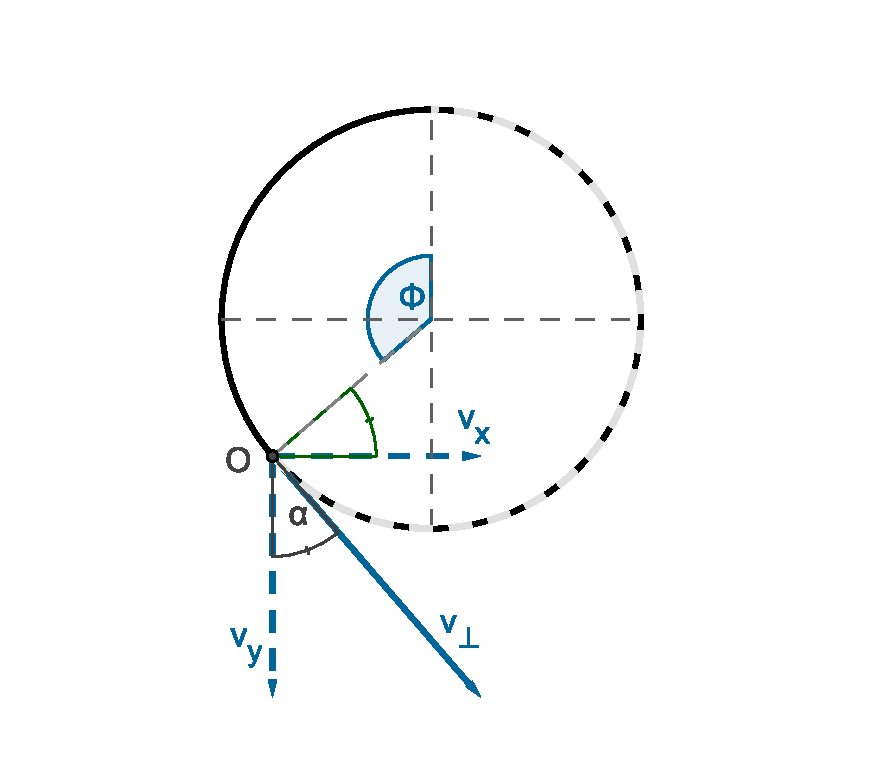
\includegraphics[width=0.5\textwidth]{figure_3.eps}
	\caption{Вылет электрона из скрещенных полей в точке O}
	\label{fig:figure1}
\end{wrapfigure}


Вылетая из скрещенных полей в момент времени $\tau$, электрон летит со скоростью $v_\perp$ в плоскости $XY$ и под действием магнитного поля вращается по окружности (также в плоскости $XY$)

Мгновенный центр окружности при $t=\tau$ будет лежать на нормали к вектору скорости.

Тогда можно найти угол $\Phi$ -- начальную фазу, набранную в скрещенных полях, из геометрии траектории - это будет $$\Phi=\frac{\pi}{2}+\alpha$$
%
\\
\\
%
Мы рассмотрели случай для горизонтально отклоняющих пластин ($E=E_x$). Понятно, что для вертикально отклоняющих пластин верно все тоже самое, но оси повернутся на $\frac{\pi}{2}$ (угол $\Phi$ будет острым) и формулы скоростей $v_x$ и $v_y$ инвертируются. 

Таким образом, для горизонтально отклоняющих пластин 

\begin{gather}
	\tg{\alpha_2}=\left|\frac{v_y(\tau)}{v_x(\tau)}\right|=\left|\frac{\cos\omega{\tau}-1}{\sin{\omega{\tau}}}\right|=\frac{1}{\tg{\alpha}}=\ctg{\alpha}\\
	\Phi=\arctg{(\ctg{\alpha})}=\frac{\pi}{2}-\arcctg{(\ctg{\alpha})}=\frac{\pi}{2}-\alpha
\end{gather}

Число фокусировок можно определить как $n=\frac{\gamma}{2\pi}$, где $\gamma$ -- весь набранный электроном угол.

Тогда
\begin{equation}
	n=\frac{\Phi+\omega\frac{l}{v_z}}{2\pi}
\end{equation}
где $l$ -- расстояние от конца пластин до экрана.

\end{document}
